\chapter{Datasety}

Data, s ktorými budeme pracovať, sú výhradne len výsledky a konečné stavy jednotlivých zápasov. 

\section{Futbal}
Pre futbal data predstavujú pre každú ligu dataset všetkých zápasov odohraných len vrámci ligy za pár posledných sezón. 
Nebudeme používať žiadne data informujúce o hráčoch, ktorí sú v oficiálnej súpiske na zápas ani data priamo len o základnej zostave na daný zápas. 
Taktiež vzhľadom na to, že tímy v jednotlivých ligách hrajú zápasy aj mimo ligy, prinajmenšom zápasy v ligovom pohári, tak nebudú použité ani informácie o oddychu pred daným zápasom, teda koľko dní pred zápasom mali zúčastnené tímy voľno.

Dataset pre každú ligu je tabuľka, kde riadky predstavujú jednotlivé zápasy zoradené podľa dátumu, v ktorom bol zápas odohraný, zostupne.
Stĺpce sú v poradí:
\begin{enumerate}
  \item Jednoznačný názov domáceho tímu (nemusí byť celý názov, stačí skrátený, ale jednoznačný a, pokiaľ možno, v celom datasete konzistentný),
  \item Jednoznačný názov hosťujúceho tímu,
  \item Id zápasu,
  \item Ligové kolo, v ktorom sa zápas odohral (0, ak sa nevie),
  \item Id domáceho tímu,
  \item Id hosťujúceho tímu,
  \item Počet gólov strelených domácim tímom v zápase,
  \item Počet gólov strelených hosťujúcim tímom v zápase,
  \item Dátum zápasu,
  \item Sezóna,
  \item Kurz na výhru domácich,
  \item Kurz na remízu,
  \item Kurz na výhru hostí.
\end{enumerate}

\noindent
\begin{figure}
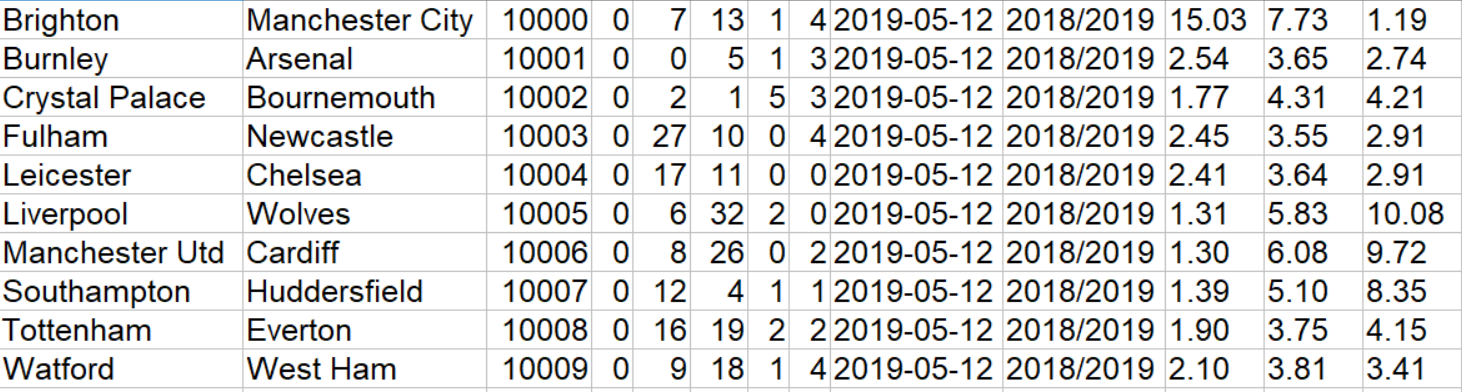
\includegraphics[width=\textwidth]{../img/eng.png}
\caption{Ukážka prvých 10 riadkov z tabuľky všetkých zápasov anglickej Premier League ilustrujúcich členenie tabuľky}
\end{figure}

Tento dataset potom predáme programu \textit{DataMaker.exe} (TODO!) písanom v jazyku C\#, ktorý pretransformuje tieto data na vstupné neuróny pre neurónovú sieť. Všetkých vstupných neurónov je 44, ich význam a poradie je popísané v sekcii Prílohy (\ref{in:foot}). 

\iffalse
\begin{multicols}{2}
\begin{enumerate}
 \item htW,
 \item htD,
 \item htL,
 \item htGFpG,	 
 \item htGApG,	 
 \item atW,	 
 \item atD,	 
 \item atL,	 
 \item atGFpG,	 
 \item atGApG,	 
 \item htHW,	 
 \item htHD,	
 \item htHL,	 
 \item htHGFpG,	 
 \item htHGApG,	 
 \item atAW,	 
 \item atAD,	 
 \item atAL,	 
 \item atAGFpG,	 
 \item atAGApG,	 
 \item hFW,	 
 \item hFD,	 
 \item hFL,	 
 \item hFGF,	 
 \item hFGA,	 
 \item aFW,	 
 \item aFD,	 
 \item aFL,	 
 \item aFGF,	 
 \item aFGA,	 
 \item MW,	 
 \item MD,	 
 \item ML,	 
 \item MGF,	 
 \item MGA,	 
 \item MhW,	 
 \item MhD,	 
 \item MhL,	 
 \item MhGF,	 
 \item MhGA,	 
 \item htLTS,	 
 \item atLTS,	 
 \item dFS,	 
 \item dFCS.
\end{enumerate}
\end{multicols}
Vysvetlivky: Prefixy: h[t] -- domáci tím, a[t] -- hosťujúci tím, F -- forma (posledných 5 zápasov), M -- posledných 5 vzájomných zápasov oboch daných tímov, Mh -- posledných 5 vzájomných zápasov oboch tímov hrané na ihrisku domáceho tímu.
Sufixy: W -- počet výher, D -- počet remíz, L -- počet prehier, GF[pG] -- počet strelených gólov prepočítaných na zápas, GA[pG] -- počet inkasovaných gólov prepočítaných na zápas, LTS -- dlhodobá sila tímu (priemerný počet bodov tímu v posledných sezónach v lige).
Ďalšie: dFS -- rozdiel v skóre formy oboch tímov, dFCS -- rozdiel v momentálnom skóre formy oboch tímov. 
Skóre formy oboch tímov je vypočítané ako počet bodov súpera v posledných 5 zápasov pre tím vynásobený počtom bodov získaných z daného zápasu. 
Momentálne skóre formy funguje podobne s výnimkou toho, že to je prepočítavané pred momentálnym zápasom, zatiaľ čo skóre sa počíta v momente ukončenia zápasu.
\fi

Skóre je pokus čo najlepšie ohodnotiť formu tímu jedným údajom. 
V sekcii (Vylepšovanie siete) (TODO!) sa budeme snažiť znížiť počet vstupných neurónov a ponechať len tie, ktoré sú dôležité. Čím väčší počet vstupných neurónov, tým väčšia je šanca, že sieť sa pokúsi medzi datami nájsť nejakú súvislosť, ktorá tam nie je, čo môže pri testovacích datach vyústiť v nesprávne výsledky (pretrénovanie dat) (TODO! cit).\\

Posledné 3 stĺpce tohto súboru predstavujú kurzy na dané výsledky. Tieto ale nie sú pri trénovaní siete využívané.

Program tiež vytvorí ďalší súbor, ktorý obsahuje testovacie data, teda data, ktoré sa nevyužívajú pri trénovaní siete, ale len pri vyhodnocovaní výsledkov. 
Tieto data sú v rovnakom poradí a musia obsahovať kurzy na dané výsledky a aj výsledok zápasu vo forme troch stĺpcov v poradí domáci, remíza, hostia, kde výsledok, ktorý nastal je ohodnotený 1, zvyšné sú 0. 
Je to potrebné pre vyhodnocovanie, pretože neurónová sieť bude mať 3 výstupné neuróny v rovnakom poradí a predikciu ohodnotí na 1.

Data v jednom súbore predstavujú pár posledných sezón a prvú polovicu sezóny 2018/2019, ktorá predstavuje všetky odohrané zápasy od začiatku sezóny až po odohratie posledného zápasu pred začiatkom kola, ktoré je numericky už v druhej polovici sezóny. 
Napríklad najvyššia anglická futbalová liga, Premier League, má 38 kôl každú sezónu, do úvahy sa bude brať posledných pár sezón pred sezónou 2018/2019 a všetky zápasy odohrané pred prvým zápasom 20. kola sezóny 2018/2019 (s výnimkou predohrávok, teda zápasov, ktoré boli preložené na dátum pred dátumom, v ktorom daný zápas figuroval v predsezónnom rozpise zápasov). 
Túto hranicu pre každú predikovanú ligu uvediem ručne do zdrojového kódu programu DataMaker.exe, pretože neviem o nejakom reálnom funkčnom algoritme, ktorý by to vedel s absolútnou istotou určiť a predstavuje to len jednu sezónu pre 5 líg.

Tento súbor je potom predaný programu v0.py (TODO!), ktorý data pripraví, vytvorí neurónovú sieť s danými parametrami (bližšie o presných parametroch v kapitole Príprava siete) a naučí ju dané data, ktoré nakoniec vyhodnotí podľa rôznych kritérií ako dôvera v daný tip alebo kurzovo vyrovnané zápasy, teda zápasy, kde na výhru domácich a vyhru hostí je dostatočne podobný kurz.

\section{Tenis}
Pre tenis budeme používať data pre najlepších 100 hráčov na začiatku každého roka v rebríčku ATP. Data v tomto prípade predstavujú zápasy z turnajov typu ATP 250, ATP 500, ATP Masters 1000, Grandslam, Finals a záverečných finálových turnajov.

Dataset je tabuľka, každý zápas predstavuje jeden riadok tabuľky, zápasy sú zoradené do turnajov od najskôr odohraných turnajov po tie najbližšie súčasnosti (ak sa obe turnaje začali a končili hrať v rovnaký deň, tak sú v ľubovoľnom poradí, nie je možné, aby poradie zmenilo nejaké data, pretože nie je možné hrať na dvoch turnajoch takéhoto typu zároveň). 
Zápasy v turnajoch sú zoradené od finále po prvé kolo, teda intuitívne opačne. 
V tomto prípade na poradí nezáleží, dôležité je, že je v tom systém. Program na spracovanie dat (ATPDataMaker.exe) si tie poradie dat upraví tak, aby mu vyhovovali. 
Stĺpce tabuľky sú v poradí:
\begin{enumerate}
  \item Názov turnaja,
  \item Počet bodov, ktoré víťaz obrdží za výhru v turnaji (ak to je neznáme, tak je tam nápis N/A)
  \item Rok, v ktorom sa turnaj odohral,
  \item Povrch kurtov na turnaji (tvrdý \textit{(Hard)}, antukový\textit{(Clay)} alebo trávnatý povrch \textit{(Grass)}),
  \item Meno víťaza zápasu,
  \item Meno hráča, ktorý zápas prehral,
  \item Kolo turnaja, v ktorom sa zápas odohral od najdôležitejšieho (1 značí finále, 2 semifinále, apod.),
  \item ID zápasu,
  \item ID víťaza (ak ID hráča je NULL, znamená to, že hráč sa doposiaľ ani raz neumiestnil v Top 100 rebríčka ATP),
  \item ID porazeného hráča,
  \item Počet setov, ktoré v zápase získal víťaz,
  \item Počet setov, ktoré v zápase získal porazený hráč,
  \item Počet hier, ktoré v zápase získal víťaz v jednotlivých setoch oddelené znakom |,
  \item Počet hier, ktoré v zápase získal porazený hráč v jednotlivých setoch oddelené znakom |,
  \item Predzápasový kurz na výhru víťaza zápasu,
  \item Predzápasový kurz na výhru porazeného hráča v zápase.
\end{enumerate}

\noindent
\begin{figure}
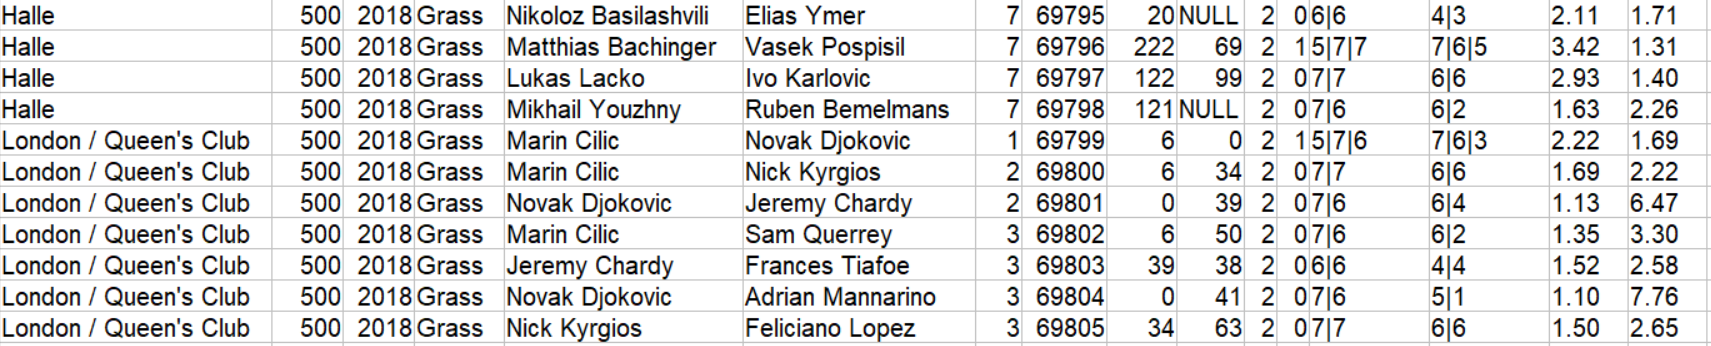
\includegraphics[width=\textwidth]{../img/atp.png}
\caption{Ukážka vybraných pár riadkov z tabuľky zápasov v okruhu ATP ilustrujúcich stĺpce a riadky.}
\end{figure}

ID hráčov sa nachádzajú v ďalšom súbore (\textit{atpranking.csv}), ktorý sa predáva aplikácii na tvorbu vstupných neurónov do neurónovej siete.
Tento súbor obsahuje ID jednotlivých hráčov, ich mená a ich poradie v koncoročných rebríčkoch hodnotenia ATP za roky 1999--2018.
Poradie berieme len ak sa hráč umiestnil na miestach 1--100.
Predzápasové kurzy môžu byť prázdne (vyplnené kurzom 0.0), ale len, ak nás na daný zápas nezaujímajú kurzy (zaujímajú nás len pre posledné dva sezóny, prvá je testovacia a druhá vyhodnocovacia sezóna).

Zápasy obsiahnuté v súbore \textit{atpresults.csv} sú len zápasy, v ktorých aspoň jeden hráč bol na konci aspoň raz v daných rokoch na miestach 1--100 v hodnotení ATP.
Predikovať sa budú len zápasy medzi takýmito hráčmi, ale kvôli rôznym výpočtom je potrebné mať všetky data o takýchto hráčoch z turnajov, ktoré sú obsiahnuté v súbore.

Tieto datasety sa potom predajú súboru \textit{ATPDataMaker.exe}, ktorý ich pretransformuje na data pre vstupné neuróny neurónových sietí. Všetkých vstupných neurónov je 37, súbor ku každému vstupnému neurónu vydá aj očakávaný výstup (1?, 2?) a pre predikovanú časť dodá aj kurzy stávkových kancelárií na daný výsledok (1B, 2B).
Poradie a význam stĺpcov je popísaný v sekcii Prílohy (\ref{in:ten}).

\iffalse
\begin{multicols}{2}
\begin{enumerate}
 \item 1W
 \item 1L
 \item 1GDpS
 \item 2W
 \item 2L
 \item 2GDpS
 \item 1FW
 \item 1FL
 \item 1FGDpS
 \item 2FW
 \item 2FL
 \item 2FGDpS
 \item 1SW
 \item 1SL
 \item 1SGDpS
 \item 2SW
 \item 2SL
 \item 2SGDpS
 \item 1SFW
 \item 1SFL
 \item 1SFGDpS
 \item 2SFW
 \item 2SFL
 \item 2SFGDpS
 \item 1MW
 \item 1ML
 \item 1MGDpS
 \item 1MSW
 \item 1MSL
 \item 1MSGDpS
 \item 1R
 \item 2R
 \item H
 \item C
 \item G
 \item dSc
 \item dSSc
 \item 1?
 \item 2?
\end{enumerate}
\end{multicols}
Vysvetlivky: Prefixy: {1,2} -- hráči, M -- vzájomné zápasy (z pohľadu hráča 1), S -- povrch (zápasy hráča na tomto povrchu), F -- forma (posledných 10 zápasov).
Suffixy: W -- počet výhier*, L -- počet prehier*, GDpS -- priemerný rozdiel v počte získaných hier v sete v prospech daného hráča, R -- poradie v rebríčku, ? -- výsledok (ak hráč vyhral - 1, inak 0)
Zvyšné: H -- tvrdý povrch, C -- antuka, G -- trávnatý povrch, dSc - rozdiel v skóre** medzi hráčmi (z pohľadu hráča 1), dSSc - rozdiel v povrchovom skóre** (z pohľadu hráča 1)\\
* - v danej sezóne, s výnimkou, ak predchádza prefix SF - povrch si uchováva formu hráča aj z minulej sezóny, ak bola braná do úvahy
** - skóre je pokus ohodnotiť silu víťazstva, berie do úvahy formu, teda posledných 10 zápasov a počíta sa ako $(150 - rank)\cdot point$, kde rank je poradie súpera v poslednom koncoročnom rebríčku ATP a point je 1, ak hráč vyhral, 0, ak vyhral súper. 
Ak súper nebol v Top 100 rebríčka ATP na konci predchádzajúceho roka, tak za jeho rank je dosadené číslo 130.
To je len preto, lebo teoreticky má dané víťazstvo hodnotu, musí byť teda nejak ohodnotené lepšie ako ľubovoľná prehra, ktorá je ohodnotená hodnotou 0.
\fi

Skóre je pokus výraznejšie ohodnotiť formu hráča ako len počtom výhier a prehier. Pri pokusoch a vylaďovaní siete budeme v sekcii (Vylepšovanie siete) (TODO!) selektovať dané vstupné neuróny podľa rôznych kritérií a vyskúšame tiež aj ako sa bude sieť správať, ak nahradíme všetky stĺpce obsahujúce data o forme rozdielom v skóre.
Teoreticky tým ušetríme 6 vstupných neurónov, príliš veľa vstupných neurónov môže viesť k rýchlejšiemu pretrénovaniu siete (TODO! cit), čomu sa budeme snažiť zabrániť selektovaním len tých dôležitých neurónov.